%-------------------------------------------------------------------------------------------------------------------------------------------------------------------------------------------------
% Section 3
%
%-------------------------------------------------------------------------------------------------------------------------------------------------------------------------------------------------
\section{Properties of Bernoulli line ensembles}\label{Section3} In this section we derive several results for non-intersecting Bernoulli bridges, which will be used in the proof of Theorem \ref{PropTightGood} in Section \ref{Section4}.


%-------------------------------------------------------------------------------------------------------------------------------------------------------------------------------------------------
% Section 3.1
%
%-------------------------------------------------------------------------------------------------------------------------------------------------------------------------------------------------
\subsection{Monotone coupling lemmas}\label{Section3.1}
 In this section we formulate two lemmas that provide couplings of two Bernoulli line ensembles of non-intersecting Bernoulli bridges on the same interval, which depend monotonically on their boundary data. Schematic depictions of the couplings are provided in Figure \ref{fig:MCL}. We postpone the proof of these lemmas until Section [Appendix]. 
\begin{figure}[ht]
\begin{center}
  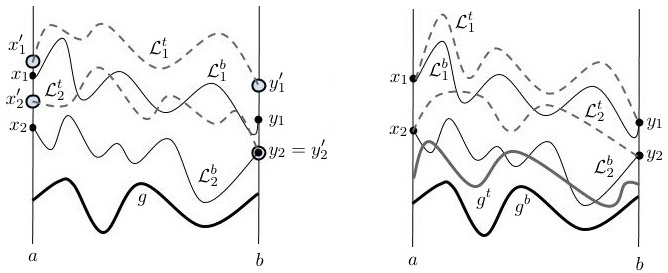
\includegraphics[scale = 0.8]{S2_1_new.jpg}
  \caption{Two diagrammatic depictions of the monotone coupling Lemma \ref{MCLxy} (left part) and Lemma \ref{MCLfg} (right part).}
  \label{fig:MCL}
  \end{center}
\end{figure}

\begin{lemma}\label{MCLxy} Assume the same notation as in Definition \ref{DefAvoidingLawBer}. Fix $k \in \mathbb{N}$, $T_0, T_1 \in \mathbb{Z}$ with $T_0 < T_1$, a function $g: \llbracket T_0, T_1 \rrbracket  \rightarrow [-\infty, \infty)$ as well as $\vec{x}, \vec{y}, \vec{x}', \vec{y}' \in \mathfrak{W}_k$. Assume that $\Omega_{avoid}(T_0, T_1, \vec{x}, \vec{y}, \infty,g)$ and $\Omega_{avoid}(T_0, T_1, \vec{x}', \vec{y}', \infty,g)$ are both non-empty. Then there exists a probability space $(\Omega, \mathcal{F}, \mathbb{P})$, which supports two $\llbracket 1, k \rrbracket$-indexed Bernoulli line ensembles $\mathfrak{L}^t$ and $\mathfrak{L}^b$ on $\llbracket T_0, T_1 \rrbracket$ such that the law of $\mathfrak{L}^{t}$ {\big (}resp. $\mathfrak{L}^b${\big )} under $\mathbb{P}$ is given by $\mathbb{P}_{avoid, Ber}^{T_0, T_1, \vec{x}', \vec{y}', \infty, g}$ {\big (}resp. $\mathbb{P}_{avoid, Ber}^{T_0, T_1, \vec{x}, \vec{y}, \infty, g}${\big )} and such that $\mathbb{P}$-almost surely we have $\mathfrak{L}_i^t(r) \geq \mathfrak{L}^b_i(r)$ for all $i = 1,\dots, k$ and $r \in \llbracket T_0, T_1 \rrbracket$.
\end{lemma}

\begin{lemma}\label{MCLfg} Assume the same notation as in Definition \ref{DefAvoidingLawBer}. Fix $k \in \mathbb{N}$,  $T_0, T_1 \in \mathbb{Z}$ with $T_0 < T_1$, two functions $g^t, g^b: \llbracket T_0, T_1 \rrbracket \rightarrow [-\infty,\infty)$ and $\vec{x}, \vec{y} \in \mathfrak{W}_k$. We assume that $g^t(r) \geq g^b(r)$ for all $r \in \llbracket T_0, T_1 \rrbracket$ and that $\Omega_{avoid}(T_0, T_1, \vec{x}, \vec{y}, \infty,g^t)$ and $\Omega_{avoid}(T_0, T_1, \vec{x}, \vec{y}, \infty,g^b)$ are both non-empty. Then there exists a probability space $(\Omega, \mathcal{F}, \mathbb{P})$, which supports two $\llbracket 1, k \rrbracket$-indexed Bernoulli line ensembles $\mathfrak{L}^t$ and $\mathfrak{L}^b$ on $\llbracket T_0, T_1 \rrbracket$ such that the law of $\mathfrak{L}^{t}$ {\big (}resp. $\mathfrak{L}^b${\big )} under $\mathbb{P}$ is given by $\mathbb{P}_{avoid, Ber}^{T_0, T_1, \vec{x}, \vec{y}, \infty, g^t}$ {\big (}resp. $\mathbb{P}_{avoid, Ber}^{T_0,T_1, \vec{x}, \vec{y}, \infty, g^b}${\big )} and such that $\mathbb{P}$-almost surely we have $\mathfrak{L}_i^t(r) \geq \mathfrak{L}^b_i(r)$ for all $i = 1,\dots, k$ and $r \in \llbracket T_0, T_1 \rrbracket$.
\end{lemma}

In plain words, Lemma \ref{MCLxy} states that one can couple two Bernoulli line ensembles $\mathfrak{L}^{t}$ and $\mathfrak{L}^{b}$ of non-intersecting Bernoulli bridges, bounded from below by the same function $g$, in such a way that if all boundary values of $\mathfrak{L}^{t}$ are above the respective boundary values of $\mathfrak{L}^{b}$, then all up-right paths of $\mathfrak{L}^{t}$ are almost surely above the respective up-right paths of $\mathfrak{L}^{b}$. See the left part of Figure \ref{fig:MCL}. Lemma \ref{MCLfg}, states that one can couple two Bernoulli line ensembles $\mathfrak{L}^{t}$ and $\mathfrak{L}^{b}$ that have the same boundary values, but the lower bound $g^t$ of $\mathfrak{L}^{t}$ is above the lower bound $g^b$ of $\mathfrak{L}^{b}$, in such a way that all up-right paths of $\mathfrak{L}^{t}$ are almost surely above the respective up-right paths of $\mathfrak{L}^{b}$. See the right part of Figure \ref{fig:MCL}.


%-------------------------------------------------------------------------------------------------------------------------------------------------------------------------------------------------
% Section 3.2
%
%-------------------------------------------------------------------------------------------------------------------------------------------------------------------------------------------------
\subsection{Properties of Bernoulli bridges}\label{Section3.2} In this section we derive several results about Bernoulli bridges, which are random up-right paths that have law $\mathbb{P}_{Ber}^{T_0, T_1, x,y}$ as in Section \ref{Section2.2}. Our results will rely on the two monotonicity Lemmas \ref{MCLxy} and \ref{MCLfg} as well as a strong coupling between Bernoulli bridges and Brownian bridges from \cite{CD} -- recalled here as Theorem \ref{KMT}.

If $W_t$ denotes a standard one-dimensional Brownian motion and $\sigma > 0$, then the process
$$B^{\sigma}_t = \sigma (W_t - t W_1), \hspace{5mm} 0 \leq t \leq 1,$$
is called a {\em Brownian bridge (conditioned on $B_0 = 0, B_1 = 0$)  with variance $\sigma^2$.}  With the above notation we state the strong coupling result we use.
\begin{theorem}\label{KMT}
Let $p \in (0,1)$. There exist constants $0 < C, a, \alpha < \infty$ (depending on $p$) such that for every positive integer $n$, there is a probability space on which are defined a Brownian bridge $B^\sigma$ with variance $\sigma^2 = p(1-p)$ and a family of random paths $\ell^{(n,z)} \in \Omega(0,n, 0, z)$ for $z = 0,\dots,n$ such that $\ell^{(n,z)}$ has law $\mathbb{P}^{0,n,0,z}_{Ber}$ and
\begin{equation}\label{KMTeq}
\mathbb{E}\left[ e^{a \Delta(n,z)} \right] \leq C e^{\alpha (\log n)^2}e^{|z- p n|^2/n}, \mbox{ where $\Delta(n,z):=  \sup_{0 \leq t \leq n} \left| \sqrt{n} B^\sigma_{t/n} + \frac{t}{n}z - \ell^{(n,z)}(t) \right|.$}
\end{equation}
\end{theorem}
\begin{remark} When $p = 1/2$ the above theorem follows (after a trivial affine shift) from \cite[Theorem 6.3]{LF} and the general $p \in (0,1)$ case was done in \cite[Theorem 4.5]{CD}. We mention that a significant generalization of Theorem \ref{KMT} for general random walk bridges has recently been proved in \cite[Theorem 2.3]{DW19}.
\end{remark}

We will use the following simple corollary of Theorem \ref{KMT} in the following to compare Bernoulli bridges with Brownian bridges. We use the same notation as in the theorem.

\begin{corollary}\label{Cheb}
	Fix $p\in (0,1)$, $\beta > 0$, and $A>0$. Suppose $|z-pn| \leq K\sqrt{n}$ for a constant $K>0$. Then for any $\epsilon > 0$, there exists $N$ large enough depending on $p,\epsilon,A,K$ so that for $n\geq N$,
	\[
	\mathbb{P}\Big(\Delta(n,z) \geq An^\beta\Big) < \epsilon.
	\]
\end{corollary}

\begin{proof}
	Applying Chebyshev's inequality and \eqref{KMTeq} gives
	\begin{align*}
	\mathbb{P}\Big(\Delta(n,z) \geq An^\beta\Big) &\leq e^{-An^\beta}\ex\Big[e^{a\Delta(n,z)}\Big] \leq C\exp\Big[-An^\beta + \alpha(\log n)^2 + \frac{|z-pn|^2}{n}\Big]\\
	&\leq C\exp\Big[-An^\beta + \alpha(\log n)^2 + K\Big].
	\end{align*}
	The conclusion is now immediate.
\end{proof}

We also state the following result regarding the distribution of the maximum of a Brownian bridge, which follows immediately from Equation (3.40) in \cite[Chapter 4]{KS}.

\begin{lemma}\label{BBmax}
	Fix $p\in (0,1)$, and let $B^\sigma$ be a Brownian bridge of variance $\sigma^2 = p(1-p)$ on $[0,1]$. Then for any $C,T> 0$,
	\[
	\mathbb{P}\Big(\max_{s\in[0,T]} B^\sigma_{s/T} \geq C\Big) = \exp\left( - \frac{2C^2}{p(1-p)}\right).
	\]
	In particular, given $\epsilon > 0$, we can choose $C$ large enough depending on $p$ so that this probability does not exceed $\epsilon$.
\end{lemma}

\begin{proof}
	Let $B^1$ be a standard Brownian bridge with variance 1 on $[0,1]$. Then $\sigma\sqrt{T}\,B^1_{s/T}$ has the same distribution as $B^\sigma_{s/T}$. Hence
	\begin{align*}
	\mathbb{P}\Big( \max_{s\in[0,T]} \sqrt{T}\,B^\sigma_{s/T} \geq T^{1/2} \Big) &= \mathbb{P}\Big( \max_{s\in[0,T]} \sqrt{T}\,B^1_{s/T} \geq C\sqrt{T}/\sigma \Big) = e^{-2(C\sqrt{T}/\sigma)^2/T} = e^{-2C^2/p(1-p)}.
	\end{align*}
	The second inequality follows from \cite[Chapter 4, (3.40)]{KS}. The second conclusion is immediate.
\end{proof}

Below we list five lemmas about Bernoulli bridges. We provide a brief informal explanation of what each result says after it is stated. All five lemmas are proved in a similar fashion. For the first four lemmas one observes that the event, whose probability is being estimated, is monotone in $\ell$. This allows by Lemmas \ref{MCLxy} and \ref{MCLfg} to replace $x,y$ in the statements of the lemmas with the extreme values of the ranges specified in each. Once the choice of $x$ and $y$ is fixed one can use our strong coupling results, Theorem \ref{KMT} and Corollary \ref{Cheb}, to reduce each of the lemmas to an analogous one involving a Brownian bridge with some prescribed variance. The latter statements are then easily confirmed as one has exact formulas for Brownian bridges, such as Lemma \ref{BBmax}.\\

\begin{lemma}\label{LemmaHalfS4} Fix $p \in (0,1)$, $T \in \mathbb{N}$ and $x, y\in \mathbb{Z}$ such that $T \geq y-x \geq 0$, and suppose that $\ell$ has distribution $\mathbb{P}^{0,T,x,y}_{Ber}$. Let $M_1, M_2 \in \mathbb{R}$ be given. Then we can find $W_0 = W_0(p,M_2 - M_1) \in \mathbb{N}$ such that for $T \geq W_0$, $x \geq M_1 T^{1/2}$, $y \geq pT + M_2 T^{1/2}$ and $s \in [0,T]$ we have
\begin{equation}\label{halfEq1S4}
\mathbb{P}^{0,T,x,y}_{Ber}\Big( \ell(s)  \geq \frac{T-s}{T} \cdot M_1 T^{1/2} + \frac{s}{T} \cdot \big(p T + M_2 T^{1/2}\big) - T^{1/4} \Big) \geq \frac{1}{3}.
\end{equation}
\end{lemma}
\begin{remark}
If $M_1, M_2 = 0$ then Lemma \ref{LemmaHalfS4} states that if a Bernoulli bridge $\ell$ is started from $(0,x)$ and terminates at $(T,y)$, which are above the straight line of slope $p$, then at any given time $s \in [0,T]$ the probability that $\ell(s)$ goes a modest distance below the straight line of slope $p$ is upper bounded by $ 2/3$.
\end{remark}
\begin{proof}
	Define $A = \lfloor M_1T^{1/2}\rfloor$ and $B = \lfloor pT + M_2 T^{1/2}\rfloor$. Then since $A\leq x$ and $B\leq y$, it follows from Lemma 3.1 that there is a probability space with measure $\mathbb{P}_0$ supporting random variables $L_1$ and $L_2$, whose laws under $\mathbb{P}_0$ are $\mathbb{P}^{0,T,A,B}_{Ber}$ and $\mathbb{P}^{0,T,x,y}_{Ber}$ respectively, and $\mathbb{P}_0$-a.s. we have $L_1\leq L_2$. Thus
	\begin{align*}
	&\mathbb{P}^{0,T,x,y}_{Ber}\Big( \ell(s)  \geq \frac{T-s}{T} \cdot M_1 T^{1/2} + \frac{s}{T} \cdot \big(p T + M_2 T^{1/2}\big) - T^{1/4} \Big)\\
	= \; & \mathbb{P}_0\Big( L_2(s)  \geq \frac{T-s}{T} \cdot M_1 T^{1/2} + \frac{s}{T} \cdot \big(p T + M_2 T^{1/2}\big) - T^{1/4} \Big)\\
	\geq \; & \mathbb{P}_0\Big( L_1(s)  \geq \frac{T-s}{T} \cdot M_1 T^{1/2} + \frac{s}{T} \cdot \big(p T + M_2 T^{1/2}\big) - T^{1/4} \Big)\\
	= \; & \mathbb{P}^{0,T,A,B}_{Ber}\Big( \ell(s)  \geq \frac{T-s}{T} \cdot M_1 T^{1/2} + \frac{s}{T} \cdot \big(p T + M_2 T^{1/2}\big) - T^{1/4} \Big).
	\end{align*}
	Since upright paths on $\llbracket 0,T\rrbracket \times \llbracket A,B\rrbracket$ are equivalent to upright paths on $\llbracket 0,T\rrbracket \times \llbracket 0, B-A\rrbracket$ shifted vertically by $A$, the last line is equal to
	\[
	\mathbb{P}^{0,T,0,B-A}_{Ber}\Big( \ell(s) + A  \geq \frac{T-s}{T} \cdot M_1 T^{1/2} + \frac{s}{T} \cdot \big(p T + M_2 T^{1/2}\big) - T^{1/4} \Big).
	\]
	Now we consider the coupling provided by Theorem \ref{KMT}. We have another probability space $(\Omega,\mathcal{F},\mathbb{P})$ supporting a random variable $\ell^{(T,B-A)}$ whose law under $\mathbb{P}$ is $\mathbb{P}^{0,T,0,B-A}_{Ber}$, and a Brownian bridge $B^\sigma$. Then 
	\begin{align*}
	&\mathbb{P}^{0,T,0,B-A}_{Ber}\Big( \ell(s) + A  \geq \frac{T-s}{T} \cdot M_1 T^{1/2} + \frac{s}{T} \cdot \big(p T + M_2 T^{1/2}\big) - T^{1/4} \Big)\\
	= \; & \mathbb{P}\Big( \ell^{(T,B-A)}(s) + A \geq \frac{T-s}{T} \cdot M_1 T^{1/2} + \frac{s}{T} \cdot \big(p T + M_2 T^{1/2}\big) - T^{1/4} \Big)\\
	= \; & \mathbb{P}\Big( \Big[\ell^{(T,B-A)}(s) - \sqrt{T} B^\sigma_{s/T} - \frac{s}{T}\cdot(B-A)\Big] + \sqrt{T}B^\sigma_{s/T} \geq -A-\frac{s}{T}\cdot(B-A) \\
	&\qquad\qquad + \frac{T-s}{T} \cdot M_1 T^{1/2} + \frac{s}{T} \cdot \big(p T + M_2 T^{1/2}\big) - T^{1/4} \Big).
	\end{align*}
	Recalling the definitions of $A$ and $B$, we can rewrite the quantity on the right hand side in the last expression and bound it by
	\begin{align*}
	\frac{T-s}{T}\cdot(M_1T^{1/2}-A) + \frac{s}{T}\cdot(pT + M_2T^{1/2} - B) - T^{1/4} &\leq  \frac{T-s}{T} + \frac{s}{T} - T^{1/4}\\
	& = -T^{1/4} + 1.
	\end{align*}
	Thus
	\begin{align*}
	&\mathbb{P}^{0,T,0,B-A}_{Ber}\Big( \ell(s) + A  \geq \frac{T-s}{T} \cdot M_1 T^{1/2} + \frac{s}{T} \cdot \big(p T + M_2 T^{1/2}\big) - T^{1/4} \Big)\\
	\geq \; & \mathbb{P}\Big( \Big[\ell^{(T,B-A)}(s) - \sqrt{T} B^\sigma_{s/T} - \frac{s}{T}\cdot(B-A)\Big] + \sqrt{T}B^\sigma_{s/T} \geq -T^{1/4} + 1 \Big)\\
	\geq \; & \mathbb{P}\Big( \sqrt{T}B^\sigma_{s/T} \geq 0 \quad \mathrm{and} \quad \Delta(T,B-A) < T^{1/4} - 1 \Big)\\
	\geq \; & \mathbb{P}\left( B^\sigma_{s/T} \geq 0 \right) - \mathbb{P}\left( \Delta(T,B-A) \geq T^{1/4} - 1 \right)\\
	= \; & \frac{1}{2} - \mathbb{P}\left( \Delta(T,B-A) \geq T^{1/4} - 1 \right).
	\end{align*}
	For the second inequality, we used the fact that the quantity in brackets is bounded in absolute value by $\Delta(T,B-A)$. The third inequality follows by dividing the event $\{B^\sigma_{s/T}\geq 0\}$ into cases and applying subadditivity. Since $|B-A-pT|\leq (M_2-M_1+1)\sqrt{T}$, Corollary \ref{Cheb} allows us to choose $W_0$ large enough depending on $p$ and $M_2-M_1$ so that if $T \geq W_0$, then the last line is bounded above by $1/2 - 1/6 = 1/3$. This proves \eqref{halfEq1S4}.
\end{proof}

\begin{lemma}\label{LemmaMinFreeS4} Fix $p \in (0,1)$, $T \in \mathbb{N}$ and $y\in \mathbb{Z}$ such that $T \geq y \geq 0$, and suppose that $\ell$ has distribution $\mathbb{P}^{0,T,0,y}_{Ber}$. Let $M > 0$ and $\epsilon > 0$ be given. Then we can find $W_1=W_1(M,p, \epsilon) \in \mathbb{N}$ and $A=A(M,p, \epsilon) > 0$ such that for $T \geq W_1$, $ y \geq p T -  MT^{1/2}$ we have
\begin{equation}\label{minFree1S4}
\mathbb{P}^{0,T,0,y}_{Ber}\Big( \inf_{s \in [ 0, T]}\big( \ell(s) -  ps \big) \leq -AT^{1/2} \Big) \leq \epsilon.
\end{equation}
\end{lemma}
\begin{remark} Roughly, Lemma \ref{LemmaMinFreeS4} states that if a Bernoulli bridge $\ell$ is started from $(0,0)$ and terminates at $(T,y)$ with $(T,y)$ not significantly lower than the straight line of slope $p$, then the event that $\ell$ goes significantly below the straight line of slope $p$ is very unlikely.
\end{remark}
\begin{proof}
	As in the previous proof, it follows from Lemma \ref{MCLxy} that
	\[
	\mathbb{P}^{0,T,0,y}_{Ber}\Big( \inf_{s \in [ 0, T]}\big( \ell(s) -  ps \big) \leq -AT^{1/2} \Big) \leq \mathbb{P}^{0,T,0,B}_{Ber}\Big( \inf_{s \in [ 0, T]}\big( \ell(s) -  ps \big) \leq -AT^{1/2} \Big),
	\]
	where $B=\lfloor pT - MT^{1/2}\rfloor$. By Theorem \ref{KMT}, there is a probability space $(\Omega,\mathcal{F},\mathbb{P})$ supporting a random variable $\ell^{(T,B)}$ whose law under $\mathbb{P}$ is that of $\ell$, and a Brownian bridge $B^\sigma$ with variance $\sigma^2 = p(1-p)$. Therefore
	\begin{align}
	&\mathbb{P}^{0,T,0,B}_{Ber}\Big( \inf_{s \in [ 0, T]}\big( \ell(s) -  ps \big) \leq -AT^{1/2} \Big) = \mathbb{P}\Big( \inf_{s \in [ 0, T]}\big( \ell^{(T,B)}(s) -  ps \big) \leq -AT^{1/2} \Big)\nonumber\\
	\leq \; & \mathbb{P}\Big( \inf_{s \in [ 0, T]}  \sqrt{T}B^\sigma_{s/T} \leq -\frac{1}{2}AT^{1/2} \Big) + \mathbb{P}\Big( \sup_{s\in [0,T]} \Big|\sqrt{T} B^\sigma_{s/T} + ps - \ell^{(T,B)}(s) \Big| \geq \frac{1}{2}AT^{1/2} \Big)\nonumber\\
	\leq \; & \mathbb{P}\Big( \max_{s\in[0,T]} B^\sigma_{s/T} \geq A/2 \Big) + \mathbb{P}\Big(\Delta(T,B) \geq \frac{1}{2}AT^{1/2} - MT^{1/2} - 1\Big). \label{MinFreeS4ineq}
	\end{align}
	For the first term in the last line, we used the fact that $B^\sigma$ and $-B^\sigma$ have the same distribution. For the second term, we used the fact that
	\begin{align*}
	\sup_{s\in[0,T]}\Big| ps - \frac{s}{T}\cdot B \Big| &\leq \sup_{s\in[0,T]}\Big| ps - \frac{pT-MT^{1/2}}{T}\cdot s \Big| + 1 = MT^{1/2} + 1.
	\end{align*}
	By Lemma \ref{BBmax}, we can take $A$ large enough depending on $p,\epsilon$ so that the first term in \eqref{MinFreeS4ineq} is $<\epsilon/2$. If we also take $A > 2M$, then since $|B-pT| \leq (M+1)\sqrt{T}$, Corollary \ref{Cheb} gives us a $W_1$ large enough depending on $M,p,\epsilon$ so that the second term is also $<\epsilon/2$ for $T\geq W_1$. Adding the two terms gives \eqref{minFree1S4}.
\end{proof}

\begin{lemma}\label{LemmaTailS4}Fix $p \in (0,1)$, $T \in \mathbb{N}$ and $x, y\in \mathbb{Z}$ such that $T \geq y-x \geq 0$, and suppose that $\ell$ has distribution $\mathbb{P}^{0,T,x,y}_{Ber}$. Let $M_1,M_2 > 0$ be given. Then we can find $W_2 = W_2(M_1,M_2,p) \in \mathbb{N}$ such that for $T \geq W_2$, $ x \geq -M_1T^{1/2}$, $ y \geq pT -  M_1T^{1/2}$ we have
\begin{equation}\label{halfEq2S4}
\mathbb{P}^{0,T,x,y}_{Ber}\bigg( \ell( T/2 )  \geq \frac{M_2T^{1/2} + p T}{2} - T^{1/4} \bigg) \geq (1/2) (1 - \Phi^{v}(M_1 + M_2) ),
\end{equation}
where $\Phi^{v}$ is the cumulative distribution function  of a Gaussian random variable with mean $0$ and variance $v = p(1-p)/4$.
\end{lemma}
\begin{remark} Lemma \ref{LemmaTailS4} states that  if a Bernoulli bridge $\ell$ is started from $(0,x)$ and terminates at $(T,y)$ with these points not significantly lower than the straight line of slope $p$, then its mid-point would lie well above the straight line of slope $p$ at least with some quantifiably tiny probability.
\end{remark}
\begin{proof}
	By Lemma \ref{MCLxy}, we have
	\begin{align*}
	\mathbb{P}^{0,T,x,y}_{Ber}\bigg( \ell( T/2 )  \geq \frac{M_2T^{1/2} + p T}{2} - T^{1/4} \bigg) &\geq \mathbb{P}^{0,T,0,B-A}_{Ber}\bigg( \ell( T/2 ) + A  \geq \frac{M_2T^{1/2} + p T}{2} - T^{1/4} \bigg)\\
	&= \mathbb{P}\bigg( \ell^{(T,B-A)}( T/2 ) + A  \geq \frac{M_2T^{1/2} + p T}{2} - T^{1/4} \bigg),
	\end{align*}
	with $A = \lfloor -M_1T^{1/2}\rfloor$, $B = \lfloor pT-M_1T^{1/2}\rfloor$, and $\mathbb{P}$, and $\ell^{(T,B-A)}$ provided by Theorem \ref{KMT}. If $B^\sigma$ is as in the theorem, we can rewrite the expression on the second line as
	\begin{align*}
	& \mathbb{P}\bigg( \bigg[\ell^{(T,B-A)}( T/2 ) -\sqrt{T}\,B^\sigma_{1/2} - \frac{B-A}{2}\bigg] + \sqrt{T}\,B^\sigma_{1/2}  \geq -A - \frac{B-A}{2} + \frac{M_2T^{1/2} + p T}{2} - T^{1/4} \bigg).
	\end{align*}
	We have
	\begin{align*}
	-A - \frac{B-A}{2} + \frac{M_2T^{1/2} + p T}{2} - T^{1/4} & \leq M_1T^{1/2} + 1 - \frac{pT-1}{2} + \frac{M_2T^{1/2} + p T}{2} - T^{1/4}\\
	&\leq (M_1 + M_2)T^{1/2} - T^{1/4} + 2.
	\end{align*}
	Thus the probability in question is bounded below by
	\begin{align*}
	& \mathbb{P}\bigg( \bigg[\ell^{(T,B-A)}( T/2 ) -\sqrt{T}\,B^\sigma_{1/2} - \frac{B-A}{2}\bigg] + \sqrt{T}\,B^\sigma_{1/2}  \geq (M_1 + M_2)T^{1/2} - T^{1/4} + 2 \bigg)\\
	\geq \; & \mathbb{P}\bigg( \sqrt{T}\,B^\sigma_{1/2} \geq (M_1 + M_2)T^{1/2} \quad \mathrm{and} \quad \Delta(T,B-A) < T^{1/4} - 2 \bigg)\\
	\geq \; & \mathbb{P}\big( B^\sigma_{1/2} \geq M_1 + M_2 \big) - \mathbb{P}\big( \Delta(T,B-A) \geq T^{1/4} - 2 \big).
	\end{align*}
	Note that $B^\sigma_{1/2} = \sigma(W_{1/2} - \frac{1}{2}W_1)$ for a standard Brownian motion $W$ on $[0,1]$. Thus $B^\sigma_{1/2}$ is Gaussian with mean 0 and variance $\sigma^2(1/2-(1/2)^2) = \sigma^2/4$. In particular, the first term in the last line is equal to
	\[
	1 - \Phi^v(M_1+M_2),
	\]
	where $\Phi^v$ is the cdf for a Gaussian random variable with mean 0 and variance $v=\sigma^2/4 = p(1-p)/4$. By Corollary \ref{Cheb}, since $|B-A-pT| \leq 1$, we can choose $W_2$ depending on $M_1,M_2$, and $p$ so that the second term is less than 1/2 the first term for $T\geq W_2$. This proves \eqref{halfEq2S4}.
\end{proof}


\begin{lemma}\label{LemmaAwayS4} Fix $p \in (0,1)$, $T \in \mathbb{N}$ and $x, y\in \mathbb{Z}$ such that $T \geq y-x \geq 0$, and suppose that $\ell$ has distribution $\mathbb{P}^{0,T,x,y}_{Ber}$. Then we can find $W_3 = W_3(p) \in \mathbb{N}$ such that for $T \geq W_3$, $ x \geq T^{1/2}$, $ y \geq pT +  T^{1/2}$
\begin{equation}\label{awayS4}
\mathbb{P}^{0,T,x,y}_{Ber}\Big( \inf_{s \in [0,T]} \big( \ell(s) -ps \big)+ T^{1/4} \geq 0 \Big) \geq \frac{1}{2} \left(1 - \exp\left(-\frac{2}{p(1-p)}\right)\right).
\end{equation}
\end{lemma}
\begin{remark} 
Lemma \ref{LemmaAwayS4} states that  if a Bernoulli bridge $\ell$ is started from $(0,x)$ and terminates at $(T,y)$ with $(0,x)$ and $(T,y)$ well above the line of slope $p$ then at least with some positive probability $\ell$ will not fall significantly below the line of slope $p$.
\end{remark}
\begin{proof}
	By Lemma \ref{MCLxy},
	\begin{align*}
	& \mathbb{P}^{0,T,x,y}_{Ber}\Big( \inf_{s \in [0,T]} \big( \ell(s) -ps \big)+ T^{1/4} \geq 0 \Big) \\
	\geq \; & \mathbb{P}^{0,T,0,B-A}_{Ber}\Big( \inf_{s \in [0,T]} \big( \ell(s) + A -ps \big)+ T^{1/4} \geq 0 \Big)\\
	= \; & \mathbb{P}\Big( \inf_{s \in [0,T]} \big( \ell^{(T,B-A)}(s) -ps \big) \geq - T^{1/4} - A \Big)\\
	\geq \; & \mathbb{P}\Big( \inf_{s \in [0,T]} \big( \ell^{(T,B-A)}(s) - \frac{s}{T}\cdot(B-A) \big) \geq - T^{1/4} - T^{1/2} + 2 \Big),
	\end{align*}
	with $A = \lfloor T^{1/2}\rfloor$, $B = \lfloor pT + T^{1/2}\rfloor$, and $\mathbb{P}$, and $\ell^{(T,B-A)}$ provided by Theorem \ref{KMT}. In the last line, we used the facts that $|A-T^{1/2}|\leq 1$ and $|p-(B-A)/T|\leq 1$. With $B^\sigma$ as in the theorem, the last line is bounded below by
	\begin{align*}
	&\mathbb{P}\Big( \inf_{s\in[0,T]} \sqrt{T}\,B^\sigma_{s/T} \geq - T^{1/2} \quad \mathrm{and} \quad \Delta(T,B-A) < T^{1/2} - 2 \Big)\\
	\geq \; & 1- \exp\left(-\frac{2}{p(1-p)}\right) - \mathbb{P}\Big( \Delta(T,B-A) \geq T^{1/2} - 2 \Big).
	\end{align*}
	In the second line, we used Lemma \ref{BBmax}. Since $|B-A-pT| \leq 1$, Corollary \ref{Cheb} allows us choose $W_3$ large enough depending on $p$ so that this term is less than $\frac{1}{2}(1-e^{-2/p(1-p)})$ for $T\geq W_3$. This implies \eqref{awayS4}.
\end{proof}


We need the following definition for our next result. For a function $f \in C[a,b]$ we define its {\em modulus of continuity} by
\begin{equation}\label{MOCS4}
w(f,\delta) = \sup_{\substack{x,y \in [a,b]\\ |x-y| \leq \delta}} |f(x) - f(y)|.
\end{equation}
\begin{lemma}\label{MOCLemmaS4}Fix $p \in (0,1)$, $T \in \mathbb{N}$ and $y\in \mathbb{Z}$ such that $T \geq y \geq 0$, and suppose that $\ell$ has distribution $\mathbb{P}^{0,T,0,y}_{Ber}$. For each positive $M$, $\epsilon$ and $\eta$, there exist a $\delta(\epsilon, \eta, M) > 0$ and $W_4 = W_4(M, p, \epsilon, \eta) \in \mathbb{N}$ such that  for $T \geq W_4$ and $|y - pT| \leq MT^{1/2}$ we have
\begin{equation}\label{MOCeqS4}
\mathbb{P}^{0,T,0,y}_{Ber}\Big( w\big({f^\ell},\delta\big) \geq \epsilon \Big) \leq \eta,
\end{equation}
where $f^\ell(u) = T^{-1/2}\big(\ell(uT) - puT\big)$  for $u \in [0,1]$.
\end{lemma}
\begin{remark}
Lemma \ref{MOCLemmaS4} states that if $\ell$ is a Bernoulli bridge that is started from $(0,0)$ and terminates at $(T,y)$ with $y$ close to $pT$ (i.e. with well-behaved endpoints) then the modulus of continuity of $\ell$ is also well-behaved with high probability.
\end{remark}
\begin{proof}
	We have
	\[
	\mathbb{P}^{0,T,0,y}_{Ber}\Big( w\big({f^\ell},\delta\big) \geq \epsilon \Big) = \mathbb{P}\Big( w\big(f^{\ell^{(T,y)}},\delta\big) \geq \epsilon \Big),
	\]
	with $\mathbb{P}$, $f^{\ell^{(T,y)}}$ as in Theorem \ref{KMT}. If $B^\sigma$ is the Brownian bridge provided by Theorem \ref{KMT}, then
	\begin{align*}
	w\big(f^{\ell^{(N,y)}},\delta\big) &= T^{-1/2} \sup_{\substack{s,t \in [0,1]\\ |s-t| \leq \delta}} \Big| \ell^{(N,y)}(sT) - psT - \ell^{(T,y)}(tT) + ptT \Big|\\
	&\leq T^{-1/2} \sup_{\substack{s,t \in [0,1]\\ |s-t| \leq \delta}} \Big(\big| \sqrt{T}\,B^\sigma_s + sy - psT - \sqrt{T}\,B^\sigma_t - ty + ptT \big|\\
	&\qquad + \big|\sqrt{T}\,B^\sigma_s + sy - \ell^{(T,y)}(sT)\big| + \big|\sqrt{T}\,B^\sigma_t + ty - \ell^{(T,y)}(tT)\big|\Big)\\
	&\leq \sup_{\substack{s,t \in [0,1]\\ |s-t| \leq \delta}} \Big| B^\sigma_s - B^\sigma_t + T^{-1/2} (y-pT)(s-t)\Big| + 2T^{-1/2}\Delta(T,y)\\
	&\leq w\big(B^\sigma,\delta\big) + M\delta + 2T^{-1/2}\Delta(T,y).
	\end{align*}
	The last line follows from the assumption that $|y-pT|\leq MT^{1/2}$. Thus
	\begin{align*}
	\mathbb{P}\Big( w\big(f^{\ell^{(N,y)}},\delta\big) \geq \epsilon \Big) &\leq \mathbb{P}\Big( w\big(B^\sigma,\delta\big) + M\delta + 2T^{-1/2}\Delta(T,y) \geq \epsilon \Big)\\
	&\leq \mathbb{P}\Big( w\big(B^\sigma,\delta\big) + M\delta \geq \epsilon/2 \Big) + \mathbb{P}\Big( \Delta(T,y) \geq \epsilon\, T^{1/2}/4 \Big).
	\end{align*}
	Corollary \ref{Cheb} gives us a $W_4$ large enough depending on $M,p,\epsilon,\eta$ so that the last term term is $\leq\eta/2$ for $T\geq W_4$. Since $B^\sigma$ is a.s. uniformly continuous on the compact interval $[0,1]$, $w(B^\sigma,\delta) \to 0$ as $\delta\to 0$. Thus we can find $\delta_0>0$ small enough depending on $\epsilon,\eta$ so that $w(B^\sigma,\delta_0) < \epsilon/2$ with probability at least $1-\eta/2$. Then with $\delta = \min(\delta_0, \epsilon/4M)$, the first term is $\leq\eta/2$ as well. This implies \eqref{MOCeqS4}.
\end{proof}


%-------------------------------------------------------------------------------------------------------------------------------------------------------------------------------------------------
% Section 3.3
%
%-------------------------------------------------------------------------------------------------------------------------------------------------------------------------------------------------
\subsection{Properties of avoiding Bernoulli line ensembles}\label{Section3.3}  In this section we derive several results about avoiding Bernoulli line ensembles, which are Bernoulli line ensembles with law $\mathbb{P}_{avoid, Ber}^{T_0,T_1, \vec{x}, \vec{y}, f, g}$ as in Definition \ref{DefAvoidingLawBer}. The lemmas we prove only involve the case when $f(r) = \infty$ for all $r \in \llbracket T_0, T_1 \rrbracket$ and we denote the measure in this case by $\mathbb{P}_{avoid, Ber}^{T_0,T_1, \vec{x}, \vec{y}, \infty, g}$. A $\mathbb{P}_{avoid, Ber}^{T_0,T_1, \vec{x}, \vec{y}, \infty, g}$-distributed random variable will be denoted by $\mathfrak{Q} = (Q_1, \dots, Q_k)$ where $k$ is the number of up-right paths in the ensemble. Our results will rely on the two monotonicity Lemmas \ref{MCLxy} and \ref{MCLfg} as well as the strong coupling between Bernoulli bridges and Brownian bridges from Theorem \ref{KMT}.


\begin{lemma}\label{LemmaDip}Fix $k, T \in \mathbb{N}$, $p \in (0,1)$, and $\vec{x}, \vec{y} \in \mathfrak{W}_k$ such that $T \geq y_i-x_i \geq 0$ for $i = 1, \dots, k$. Suppose that $g: \llbracket 0, T \rrbracket \rightarrow [-\infty, \infty)$ is such that $g(0) \leq x_k$, $g(T) \leq y_k$ and $g(i +1 ) = g(i) $ or $g(i+1) = g(i) +1$ for $i = 0, \dots, T-1$. Suppose that $\ell$ has distribution $\mathbb{P}^{0,T,\vec{x},\vec{y}, \infty ,g}_{avoid,Ber}$ as in Definition \ref{DefAvoidingLawBer} (notice this distribtuion is well-defined by Lemma \ref{LemmaWD}). Let $M_1,M_2, M_3 > 0$ be given. Then we can find $W_5 = W_5(M_1,M_2, M_3, p) \in \mathbb{N}$ such that for $T \geq W_5$, $ x_1 \leq M_1T^{1/2}$, $ y_1 \leq pT -  M_2 T^{1/2}$ and $g$ satisfying $g(r) \leq p \cdot r - M_3T^{1/2}$ for $r \in \llbracket 0, T\rrbracket$ we have
\begin{equation}\label{eqDip}
\mathbb{P}^{0,T,\vec{x},\vec{y}, \infty ,g}_{avoid,Ber}\bigg( Q_1( T/2 )  \leq k (M_1+1)T^{1/2} +  \frac{ (M_1 - M_2)T^{1/2} + p T}{2}  \bigg) \geq [Something].
\end{equation}
\end{lemma}
\begin{proof}
\end{proof}
